%!TEX encoding = UTF-8 Unicode
%!TEX root = ../lect-week06.tex

%%%

\Subsection{Vad är en klass?}

\begin{Slide}{Vad är en klass?}
\begin{itemize} 
\item En klass är en mall för att skapa objekt. 
\item Objekt skapas med \code{new Klassnamn} och kallas för  \Emph{instanser} av klassen \code{Klassnamn}.
\item En klass innehåller medlemmar \Eng{members}: 
  \begin{itemize} 
  \item \Emph{attribut}, kallas även fält \Eng{field}: \code{val}, \code{lazy val}, \code{var} 
  \item \Emph{metoder}, kallas även operationer: \code{def}
  \end{itemize}
\item Varje instans har sin uppsättning värden på attributen (fälten).
\end{itemize}

\end{Slide}


\ifkompendium\else


\begin{Slide}{Vad är en klass?}\SlideFontSmall
Metafor: En klass liknar en \Emph{stämpel}
\begin{figure}
\centering
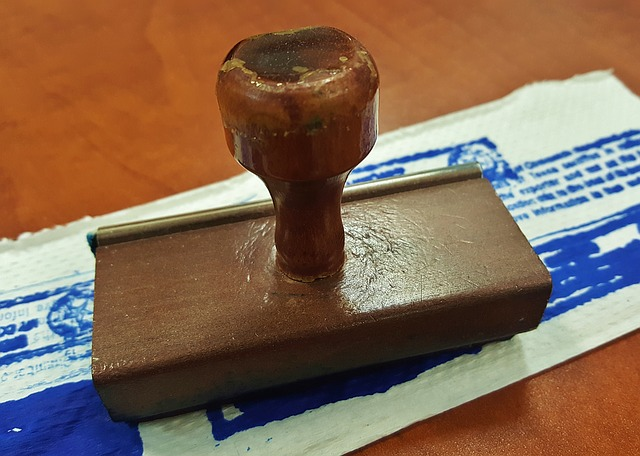
\includegraphics[width=0.5\textwidth]{../img/stamp}
\end{figure}
\begin{itemize}
\item En stämpel kan tillverkas -- motsvarar deklaration av klassen. 
 \item Det händer inget förrän man stämplar -- motsvarar \code{new}.
\item Då skapas avbildningar -- motsvarar instanser av klassen.


\end{itemize}
\end{Slide}


\begin{Slide}{Syntax för klassdeklarationer}
Klassens ''anatomi''
\end{Slide}


\begin{Slide}{Exempel: Klassen Complex}\small
%TODO:
%  \begin{itemize} 
%  \item Bygg upp \code{case class Complex(re: Double, im: Double)} steg för steg inspirerat av Pins3ed kap 6 i likhet med hur de gör med Rational
%  \item Illustrera följande begrepp: this (behövs i max(that)), method overloading behövs för att plussa med både Complex och Double
%  \item Till fördjupningsövning: dekorera Double med metoderna im och re samt (Double, Double) med metoden ir (för irrational) med implicit klass
%  \item Till extrauppgift: implementera klassen Polar(r, fi) med polära koordinater \url{https://sv.wikipedia.org/wiki/Pol%C3%A4ra_koordinater}
%  \end{itemize}
\end{Slide}


\Subsection{Instansiering: \texttt{new}}

\begin{Slide}{Instansiering med \texttt{new}}
\end{Slide}

\begin{Slide}{Instansiering med fabriksmetod}
\end{Slide}

\begin{Slide}{Instansiering med default-argument}
\end{Slide}

\begin{Slide}{Instansiering med alternativa fabriksmetoder}
\end{Slide}

\begin{Slide}{Förändringsbar eller oföränderlig?}
\end{Slide}


\Subsection{Referens saknas: \texttt{null}}

\begin{Slide}{Referens saknas: \texttt{null}}
\end{Slide}


\begin{Slide}{Konstruktor}
\end{Slide}

\begin{Slide}{Skräpsamling}
Destruktor
\end{Slide}

\Subsection{Synlighet}

\begin{Slide}{Synlighet}
definiera/förklara:
private
private[this]
\end{Slide}

\begin{Slide}{Kompanjonsobjekt}
\end{Slide}


\begin{Slide}{Synlighet av klassparametrar i klasser \& case-klasser}\SlideFontSmall
\code{private[this]} är \Alert{ännu} mer privat än \code{private} 
\begin{Code}
class Hemlis(private val hemlis: Int) {
  def ärSammaSom(annan: Hemlis) = hemlis == annan.hemlis   // Funkar!
}

class Hemligare(private[this] val hemlis: Int) {
  def ärSammaSom(annan: Hemligare) = hemlis == annan.hemlis //KOMPILERINGSFEL
}
\end{Code}
Vad händer om man inte skriver något? Olika för klass och case-klass:
\begin{Code}
class Hemligare(hemlis: Int) { // motsvarar private[this] val
  def ärSammaSom(annan: Hemligare) = hemlis == annan.hemlis //KOMPILERINGSFEL
}

case class InteHemlig(seMenInteRöra: Int) { // blir automatiskt val 
  def ärSammaSom(annan: InteHemlig): Boolean = 
    seMenInteRöra == annan.seMenInteRöra 
}

\end{Code}
\end{Slide}


\Subsection{Klasser i Java}

\begin{Slide}{Klasser i Java}
\end{Slide}

\begin{Slide}{Statiska medlemmar}
\end{Slide}


\Subsection{Getters och setters}

\begin{Slide}{Getters och setters i Java}
\end{Slide}

\begin{Slide}{Getters och setters i Scala}
\end{Slide}

\begin{Slide}{Ändra attributrepresentation utan att påverka existerande kod}
Complex som polära koordinater i Java med privat attribut
Complex som polära koordinater med publika attribut om man har enhetlig access
\end{Slide}


\Subsection{Implementation saknas: ???}

\begin{Slide}{Implementation saknas: ???}
\end{Slide}


\fi

